\documentclass{beamer}
\mode<presentation>

%% packages
\usepackage{beamerthemeshadow}
\usepackage{xcolor}
\usepackage[english]{babel}
\usepackage[latin1]{inputenc}
\usepackage{times}
\usepackage[T1]{fontenc}
\usepackage{wrapfig}
\usepackage{color}
\usepackage{graphicx}
\usepackage{subfigure}
\usepackage{multirow}
\usepackage{amsmath}
\usepackage{tikz}
\usetikzlibrary{automata,positioning,arrows}
\usepackage{etoolbox}
\usepackage{hyperref}

%% The Beamer class comes with a number of default slide themes which change the colors and layouts of slides. For more details go to  http://deic.uab.es/~iblanes/beamer_gallery/
%\usetheme{default}
%\usetheme{AnnArbor} % Yellow colored theme, 3 parition in footer
%\usetheme{Antibes}  % Blue shadowed theme, 2 partition in footer
%\usetheme{Bergen}   % left side navigation, 2 partition in footer
%\usetheme{Berkeley}
%\usetheme{Berlin}   % bottom vertical partition, horizontal top navigation
%\usetheme{Boadilla} % light blue navigation, 3 partition at bottom
\usetheme{CambridgeUS} % red color cool theme, 3 partition
%\usetheme{Copenhagen}
%\usetheme{Darmstadt}
%\usetheme{Dresden}
%\usetheme{EastLansing} % cool green colored theme
%\usetheme{Frankfurt}
%\usetheme{Goettingen}
%\usetheme{Hannover}
%\usetheme{Ilmenau}
%\usetheme{JuanLesPins}
%\usetheme{Luebeck}
%\usetheme{Madrid}
%\usetheme{Malmoe}
%\usetheme{Marburg}
%\usetheme{Montpellier}
%\usetheme{PaloAlto}
%\usetheme{Pittsburgh}
%\usetheme{Rochester}
%\usetheme{Singapore}
%\usetheme{Szeged}
%\usetheme{Warsaw}

%% As well as themes, the Beamer class has a number of color themes for any slide theme.
%\usecolortheme{albatross}
%\usecolortheme{beaver}
%\usecolortheme{beetle}
%\usecolortheme{crane}
%\usecolortheme{dolphin}
%\usecolortheme{dove}
%\usecolortheme{fly}
%\usecolortheme{lily}
%\usecolortheme{orchid}
%\usecolortheme{rose}
%\usecolortheme{seagull}
%\usecolortheme{seahorse}
%\usecolortheme{whale}
%\usecolortheme{wolverine}

%% font themes
%\usefonttheme{structurebold}
%\usefonttheme{professionalfonts}
%\usefonttheme{structuresmallcapsserif}
%\usefonttheme{serif}
\usefonttheme{structureitalicserif}

%% color definition
\definecolor{darkred}{RGB}{140,0,47}

%% custom color
%\setbeamercolor{alerted text}{fg=orange}
%\setbeamercolor{background canvas}{bg=white}
%\setbeamercolor{block body alerted}{bg=normal text.bg!90!black}
%\setbeamercolor{block body}{bg=normal text.bg!90!black}
%\setbeamercolor{block body example}{bg=normal text.bg!90!black}
%\setbeamercolor{block title alerted}{use={normal text,alerted text},fg=alerted text.fg!75!normal text.fg,bg=normal text.bg!75!black}
%\setbeamercolor{block title}{bg=blue}
%\setbeamercolor{block title example}{use={normal text,example text},fg=example text.fg!75!normal text.fg,bg=normal text.bg!75!black}
%\setbeamercolor{fine separation line}{}
%\setbeamercolor{frametitle}{fg=brown}
%\setbeamercolor{item projected}{fg=black}
%\setbeamercolor{normal text}{bg=black,fg=yellow}
%\setbeamercolor{palette sidebar primary}{use=normal text,fg=normal text.fg}
%\setbeamercolor{palette sidebar quaternary}{use=structure,fg=structure.fg}
%\setbeamercolor{palette sidebar secondary}{use=structure,fg=structure.fg}
%\setbeamercolor{palette sidebar tertiary}{use=normal text,fg=normal text.fg}
%\setbeamercolor{section in sidebar}{fg=brown}
%\setbeamercolor{section in sidebar shaded}{fg= grey}
%\setbeamercolor{separation line}{}
%\setbeamercolor{sidebar}{bg=red}
%\setbeamercolor{sidebar}{parent=palette primary}
\setbeamercolor{structure}{fg=darkred}
%\setbeamercolor{subsection in sidebar}{fg=brown}
%\setbeamercolor{subsection in sidebar shaded}{fg= grey}
%\setbeamercolor{title}{fg=brown}
%\setbeamercolor{titlelike}{fg=brown}

%% control header
\setbeamertemplate{headline}{}

%% control footer
%\setbeamertemplate{footline}
%\setbeamertemplate{footline}[page number]

%% removes navigation symbol
%\setbeamertemplate{navigation symbols}{}

%% bibilography settings
\setbeamertemplate{frametitle continuation}[from second]
\setbeamercolor*{bibliography entry title}{fg=black}
\setbeamercolor*{bibliography entry author}{fg=black}
\setbeamercolor*{bibliography entry location}{fg=black}
\setbeamercolor*{bibliography entry note}{fg=black}

%% same slide number for continuation slides
\newcounter{multipleslide}
\makeatletter
\newcommand{\multipleframe}
{
	\setcounter{multipleslide}{\value{framenumber}}
	\stepcounter{multipleslide}
	\patchcmd{\beamer@@tmpl@footline}
	{\insertframenumber}
	{\themultipleslide}
	{}
	{}
}
\newcommand{\restoreframe}
{
	\patchcmd{\beamer@@tmpl@footline}
	{\themultipleslide}
  	{\insertframenumber}
	{}
	{}
	\setcounter{framenumber}{\value{multipleslide}}
}
\makeatother

%% title page
\title[Erlang Distributed File System (eDFS)]
{
	BTP stage-I \\
	Erlang Distributed File System (eDFS)
}
\author[Aman Mangal \\ (IIT Bombay)]
{	\sffamily
	\textbf{By:} Aman Mangal \\
	\textbf{Advisor:} Prof G. Sivakumar \\
	\textbf{Examiner:} Prof Umesh Bellur \\
	IIT Bombay
}
\date{\today}

\begin{document}
\begin{frame}
\addtocounter{framenumber}{-1}
\begin{figure}
    
\includegraphics[width=2.3cm]{images/iitb}
    \hspace*{0.8cm}
    
\includegraphics[width=2.3cm]{images/erlang}
\end{figure}
\titlepage
\end{frame}

\begin{frame}\frametitle{Presentation Outline}
\tableofcontents
\end{frame}


\section{Distributed File System}
\begin{frame}{Distributed File System}
\addtocounter{framenumber}{-1}
\tableofcontents[currentsection]
\end{frame}

\subsection{Introduction}
\begin{frame}{Introduction}
\begin{itemize}
\item Extension of file system
\item Exploits multiple nodes communicating over network
\item Provides large data storage, high availability and reliability of data
\item Useful for applications processing large amount of data such as Search engines, data mining applications
\end{itemize}
\end{frame}

\subsection{Related Work}
\begin{frame}{Related Work}
\begin{itemize}
\item \textbf{Old:} Unix United, Locus, Sun NFS, Sprite, Andrew
\begin{itemize}
\item Part of Operating System just like file system
\item Focus on sharing of resources
\item Treat failures as exceptions
\end{itemize}
\item \textbf{Modern:} Panasas, GFS, HDFS, TidyFS
\begin{itemize}
\item Cluster based architecture
\item Metadata stored separately, decoupling control from data path
\item Component failures as norm, therefore, fault tolerant
\end{itemize}
\item \textbf{Other:} GreenHDFS
\begin{itemize}
\item Go green, focus on energy conservation
\end{itemize}
\end{itemize}
\end{frame}

\subsection{Issues with Existing Solutions}
\begin{frame}{Issues with Existing Solutions}
\begin{itemize}
\item Scalability and Fault Tolerance issues
\item Metadata server is single point of failure
\item HDFS solutions for scalability (Not yet implemented)
\begin{itemize}
\item Multiple clusters in one DFS
\item Storing partial metadata in memory
\end{itemize}
\item Polling based fault tolerance mechanism
\item Stateful servers, requires garbage collection of cached data and processes
\item Requires more powerful primitives to solve the problem
\end{itemize}
\end{frame}


\section{Problem Statement}
\begin{frame}{Problem Statement}
\addtocounter{framenumber}{-1}
\tableofcontents[currentsection]
\end{frame}

\subsection{Erlang}
\begin{frame}{Erlang}
\begin{itemize}
\item Highly concurrent pure functional programming language
\item Runs on BEAM vm, its own scheduler, garbage collector
\item No shared memory, asynchronous message passing
\item Fast creation \& destroying of process
\item Follows event based protocols, allows linking of processes
\item OTP principles separate sequential program with concurrent part
\end{itemize}
\end{frame}

\subsection{Motivation}
\begin{frame}{Motivation}
\begin{itemize}
\item Leverage distributed capabilities of Erlang
\item Focus on scalability and fault tolerance
\item Understand more issues with a distributed system
\item Problem statement
\begin{itemize}
\item Develop a basic file system in Erlang
\item Look into scalability and fault tolerance capabilities of eDFS
\end{itemize}
\end{itemize}
\end{frame}


\section{Erlang Distributed File System}
\begin{frame}{Erlang Distributed File System}
\addtocounter{framenumber}{-1}
\tableofcontents[currentsection]
\end{frame}

\subsection{Assumptions}
\begin{frame}{Assumptions}
\begin{itemize}
\item Runs on commodity servers
\item Trusted nodes and network
\item Component failures as norm not exceptions
\item General purpose workload but DFS optimized for high throughput, sequential I/O
\item UNIX like interface for client to communicate
\end{itemize}
\end{frame}

\begin{frame}{Architecture}
\begin{columns}[onlytextwidth]
  \begin{column}{0.6\textwidth}
      \begin{itemize}
      \item Cluster based architecture
      \item Single master, multiple worker nodes
      \item Any number of client servers
      \item Multiple writer multiple reader model
      \item Based on Erlang message passing \& socket based TCP communication
      \item Fully network, location transparent
      \item Reliable, highly concurrent, scalable \& fault tolerant
      \end{itemize}
  \end{column}
  \begin{column}{0.4\textwidth}
      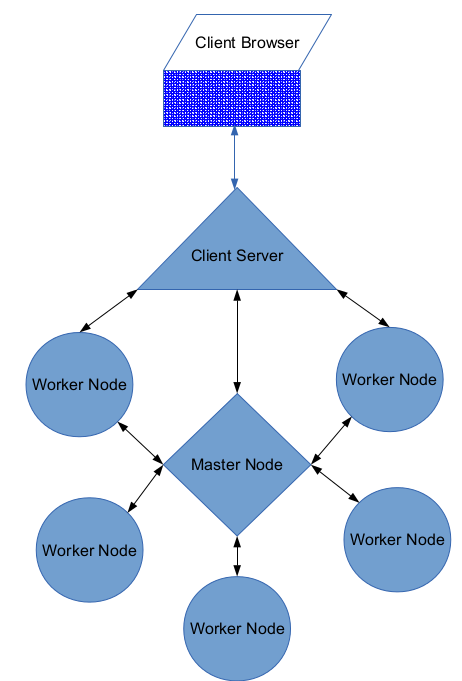
\includegraphics[scale=0.3]{images/design}
  \end{column}
\end{columns}
\end{frame}

\subsection{Master, Worker \& Client}
\begin{frame}{Master Node}
\begin{columns}
    \begin{column}{0.7\textwidth}
        \begin{itemize}
        \item Handles metadata using Mnesia database in RAM \& disk both
        \item Monitors workers through Heartbeats
        \item Namespace management
        \item Ensure replication factor is met
        \item Journal \& Checkpoint creation
        \end{itemize}
    \end{column}
    \begin{column}{0.3\textwidth}
        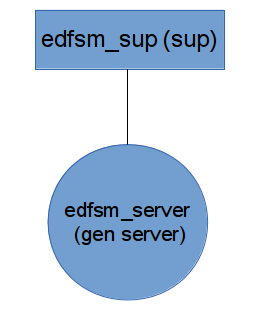
\includegraphics[scale=0.4]{images/master_otp_layout}
    \end{column}
\end{columns}
\end{frame}

\begin{frame}{Worker Node}
\begin{columns}
    \begin{column}{0.5\textwidth}
        \begin{itemize}
        \item Performs handshake with master on start up
        \item Implemented as Finite State Machine (4 States)
        \begin{enumerate}
        \item ReadWrite (normal state)
        \item ReadOnly \item Distress
        \item Unavailable
        \end{enumerate}
        \item Provides TCP servers for client to communicate
        \end{itemize}
    \end{column}
    \begin{column}{0.5\textwidth}
        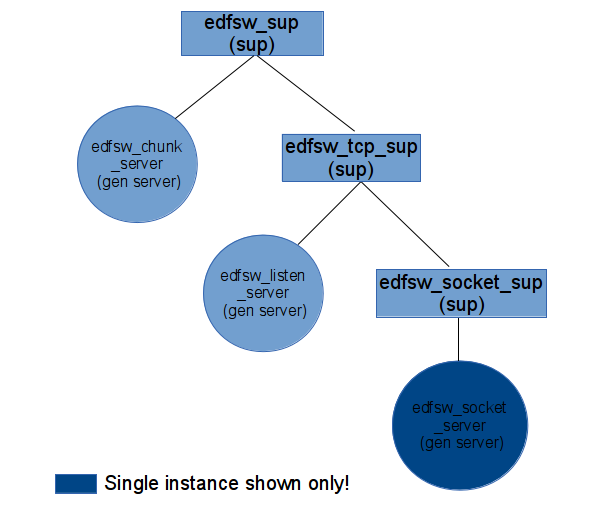
\includegraphics[scale=0.3]{images/worker_otp_layout}
    \end{column}
\end{columns}
\end{frame}

\begin{frame}{Client Server}
\begin{columns}
    \begin{column}{0.5\textwidth}
        \begin{itemize}
        \item Provides UNIX like interface for clients to manipulate files
        \item Separate file handlers for files
        \item Cache while writing and reading data from worker node
        \end{itemize}
    \end{column}
    \begin{column}{0.5\textwidth}
        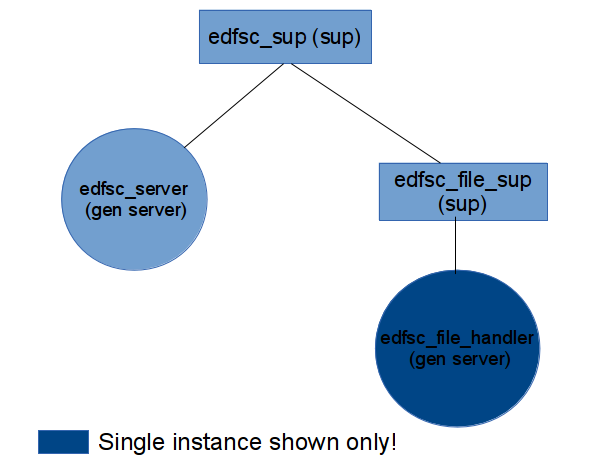
\includegraphics[scale=0.3]{images/client_otp_layout}
    \end{column}
\end{columns}
\end{frame}

\subsection{Features}
\begin{frame}{Garbage Collector}
\begin{itemize}
\item Each worker implements a garbage collector process
\item Periodic scans through stored data and metadata
\item Deletes/updates stale replicas of blocks
\item Verifies checksum of stored blocks
\item Sends an updated list of stored blocks to master node
\end{itemize}
\end{frame}

\begin{frame}{Create a New File}
    \begin{figure}[h]
    \begin{tikzpicture}[shorten >=2pt,node distance=4cm,on grid,auto]
        \tikzstyle{every state}=[draw=blue!50,very thick,fill=blue!20]
        \node[state] (Rd) {Client};
        \node[state] (Rn) [right=7.5cm =of Rd] {Master};
        \path[->]
        (Rd) edge node[anchor=center, above] {\{createFile, "/home/numbers.txt", 3\}} (Rn);
    \end{tikzpicture}
    \end{figure}
\begin{itemize}
\item Client's actions-
\begin{itemize}
\item Sends \textit{create file} request to master node
\item Synchronous request using Erlang message passing
\item Specifies replication factor if different than 3
\end{itemize}
\item Master's actions
\begin{itemize}
\item Create the path if doesn't exist
\item Make an entry for the file
\end{itemize}
\end{itemize}
\end{frame}

\begin{frame}[allowframebreaks]{Append File}
\multipleframe
\begin{itemize}
\item Client node sends an open file request to master node
\begin{figure}[h]
    \begin{tikzpicture}[shorten >=2pt,node distance=4cm,on grid,auto]
        \tikzstyle{every state}=[draw=blue!50,very thick,fill=blue!20]
        \node[state] (Rd) {Client};
        \node[state] (Rn) [right=7.5cm =of Rd] {Master};
        \path[->]
        (Rd) edge node[anchor=center, above] {\{openFile, "/home/numbers.txt", a\}} (Rn);
    \end{tikzpicture}
    \end{figure}
\item Master node replies with all the replicas and chunk id
    \begin{figure}[h]
    \begin{tikzpicture}[shorten >=2pt,node distance=4cm,on grid,auto]
        \tikzstyle{every state}=[draw=blue!50,very thick,fill=blue!20]
        \node[state] (Rd) {Client};
        \node[state] (Rn) [right=7cm =of Rd] {Master};
        \path[<-]
        (Rd) edge node[sloped, anchor=center, above, text width=6cm] {\{"/home/numbers.txt", Replicas, ChunkId, MaxSize\}} (Rn);
    \end{tikzpicture}
    \end{figure}
    \item Replicas contains all replicas including primary replica with their IP address and port
    \item MaxSize is maximum amount of data which is allowed to be written on the given chunk
    \item Client connects to primary replica on TCP/IP socket
    \begin{figure}[h]
    \begin{tikzpicture}[shorten >=2pt,node distance=4cm,on grid,auto]
        \tikzstyle{every state}=[draw=blue!50,very thick,fill=blue!20]
        \node[state] (Rd) {Client};
        \node[state] (Rn) [right=8cm =of Rd] {Worker};
        \path[->]
        (Rd) edge node[anchor=center, above] {\{openChunk, ChunkId, RestReplicas\}} (Rn);
    \end{tikzpicture}
    \end{figure}
    \item Client caches the data and sends in packets of size MTU (4KB) or after time out occurs
    \begin{figure}[h]
    \begin{tikzpicture}[shorten >=2pt,node distance=4cm,on grid,auto]
        \tikzstyle{every state}=[draw=blue!50,very thick,fill=blue!20]
        \node[state] (Rd) {Client};
        \node[state] (Rn) [right=8cm =of Rd] {Worker};
        \path[->]
        (Rd) edge node[anchor=center, above] {\{writeData, Data, CheckSum\}} (Rn);
    \end{tikzpicture}
    \end{figure}
    \framebreak
    \item Client node closes the file and socket when
    \begin{figure}[h]
    \begin{tikzpicture}[shorten >=2pt,node distance=4cm,on grid,auto]
        \tikzstyle{every state}=[draw=blue!50,very thick,fill=blue!20]
        \node[state] (Rd) {Client};
        \node[state] (Rn) [right=8cm =of Rd] {Master};
        \path[->]
        (Rd) edge node[anchor=center, above, text width=6cm] {\{writtenData, FileName, a, ChunkId, SentSize, WantNew\}} (Rn);
    \end{tikzpicture}
    \end{figure}
    \begin{itemize}
    \item Client requests to close the file, \textbf{WantNew=false}
    \item Data written crosses the value of \textit{MaxSize}, \textbf{WantNew=true}
    \item Repeats from setting up the socket again
    \end{itemize}
\end{itemize}
\framebreak
\begin{columns}
    \begin{column}{0.4\textwidth}
        \begin{itemize}
        \item Worker node sets up a pipeline by connecting all the replicas
        \item Primary forwards all the requests to other replicas in the pipeline
        \end{itemize}
    \end{column}
    \begin{column}{0.6\textwidth}
        \begin{figure}[h]
            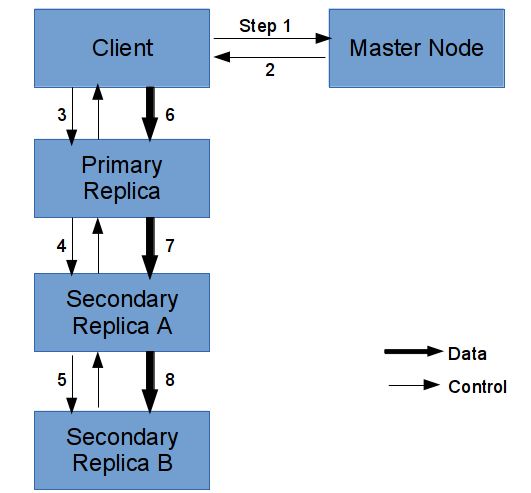
\includegraphics[scale=0.4]{images/append_pipeline}
        \end{figure}
    \end{column}
\end{columns}
\end{frame}
\restoreframe

\begin{frame}{Fault Tolerance}
\begin{itemize}
\item What if any of worker fails
\begin{itemize}
\item Pipeline is broken
\item Try again to set up new pipeline removing the failed worker
\item Based on timestamp, the failed worker will update data whenever it comes up again
\end{itemize}
\item What if client fails
\begin{itemize}
\item Timeout will occur and all the TCP server processes will be closed
\item No need for explicit garbage collection of processes
\end{itemize}
\item Combination of Stateful \& Stateless servers!
\end{itemize}
\end{frame}


\section{Future Work}
\begin{frame}{Future Work}
\begin{itemize}
\item Complete basic DFS
\item Concurrent write \& append operations
\item Explicit locking mechanism
\item Truly distributed implementation of metadata server
\item Checkpoint, snapshots and logging mechanism
\item Map reduce framework
\end{itemize}
\end{frame}


\section{Resources}
\begin{frame}{Resources}
\begin{itemize}
\item \href{http://www.cse.iitb.ac.in/~amanmangal/External/btp/}{Project Home Page} \url{www.cse.iitb.ac.in/~amanmangal/External/btp/}
\item \href{https://github.com/mangalaman93/eDFS}{Code hosted on Github} \url{github.com/mangalaman93/eDFS}
\item \href{http://www.cse.iitb.ac.in/~amanmangal/External/btp/edfs.pdf}{Report} \url{www.cse.iitb.ac.in/~amanmangal/External/btp/edfs.pdf}
\end{itemize}
\end{frame}


\section{References}
\multipleframe
\begin{frame}[allowframebreaks]
\frametitle{References}
\begin{thebibliography}{99}
\bibitem{erlang}
  http://www.erlang.org/

\bibitem{bert}
  http://bert-rpc.org/

\bibitem{armstrong}
  \textsc{Joe Armstrong},
  "Making Reliable Distributed Systems in the Presence of Software Errors",
  \emph{A Dissertation submitted to the Royal Institute of Technology Stockholm}
  Sweden, December 2003.

\bibitem{blog_joe}
  \textsc{Joe Armstrong},
  "What's All the Fuss About Erlang",
  \emph{http://pragprog.com/articles/erlang},
  2007.

\bibitem{old_dfs}
  \textsc{Eliezer levy, Abraham silberschatz},
  "Distributed File Systems: Concepts and Examples",
  \emph{ACM Computing Surveys, Vol. 22, No. 4},
  December 1990.

\bibitem{panasas}
  \textsc{Nagle D., Serenyi D., Matthews A.},
  "The Panasas ActiveScale Storage Cluster: Delivering Scalable High Bandwidth Storage",
  \emph{Proceedings of the 2004 ACM/IEEE conference on Supercomputing, pp. 53-},
  2004.

\bibitem{ghemawat03}
  \textsc{Sanjay Ghemawat, Howard Gobioff and Shun-Tak Leung},
  "The Google file system",
  \emph{In SOSP '03: Proceedings of the nineteenth ACM symposium on Operating systems principles}
  New York, NY, USA, 2003

\bibitem{hadoop}
  \textsc{Konstantin Shvachko, Hairong Kunag, Sanjay Radia and Robert Chansler},
  "The Hadoop Distributed File System"
  Sunnyvale, California USA

\bibitem{tidyfs}
  \textsc{Dennis Fetterly, Maya Haridasan, Michael Isard and Swaminathan Sundararaman},
  "TidyFS: A Simple and Small Distributed File System".
  \emph{Microsoft Research Technical Report},
  MSR-TR-20110-24

\bibitem{zhou}
  \textsc{Yuduo Zhou},
  "Large Scale Distributed File System Survey",
  \emph{Indiana University Bloomington}

\bibitem{maurya}
  \textsc{Maurya M., Oza C., Shah K.}
  "A Review of Distributed File Systems"
  \emph{MPSTME, SVKM's NMISMS University}
  Vile Parle West, Mumbai-56

\bibitem{satya}
  \textsc{Satyanarayanan, M.},
  "A Survey of Distributed File Systems",
  \emph{Technical Report CMU-CS-89- 116, Department of Computer Science, Camegie Mellon University},
  1989.

\bibitem{thanh}
  \textsc{Tran Doan Thanh, Subaji Mohan, Eunmi Choi, SangBum Kim, Pilsung Kil}
  "A Taxonomy and Survey of Distributed File System"
  \emph{School of Business IT, Kookmin University}
  Seoul, Korea, 2008

\bibitem{ghemawat08}
  \textsc{Dean Jeffrey, Ghemawat Sanjay}
  "MapReduce: simplified data processing on large clusters"
  \emph{Communications of the ACM}
  New York, NY, USA, January 2008

\bibitem{eric}
  \textsc{Logan Martin, Merritt Eric and Carlsson Richard}
  "Erlang and OTP in Action",
  2010
\end{thebibliography}
\end{frame}
\restoreframe

\begin{frame} \frametitle{Thank you}
\Huge{\centerline{\color{darkred}Questions?}}
\end{frame}

\end{document}
